%%%%%%%%%%%%%%%%%%%%%%%%%%%%%%%%%%%%%%%
% Main Macro of arbitary documents
% Name : Yuki Sakurai
% e-mail : yuki.sakurai@cern.ch
%%%%%%%%%%%%%%%%%%%%%%%%%%%%%%%%%%%%%%%
\documentclass[11pt]{article}

% \setlength{\oddsidemargin}{0mm}

% Change Paper Geometry
\usepackage[top=30truemm,bottom=30truemm,left=25truemm,right=25truemm]{geometry}

%%%% packages
\usepackage{physics}
\usepackage{lineno}
\usepackage[dvipdfmx]{graphicx,color}
\usepackage{setspace}
\usepackage{wrapfig}
\usepackage{amsmath}
\usepackage{epsfig}
\usepackage{bm}
\usepackage{times}
\usepackage{color}
\usepackage{fancybox}
\usepackage{comment}
\usepackage{multirow}
\usepackage{color}
\usepackage{eso-pic}
\usepackage{rotating}
\usepackage{cite}
\usepackage{url}
\usepackage{subfigure}
\usepackage{array}

% newcommand
\newcommand{\fulltoday}{\ifcase\month\or
    Jan.\or Feb.\or Mar.\or Apr.\or May\or Jun.\or
    Jul.\or Aug.\or Sep.\or Oct.\or Nov.\or Dec.\fi
    \space\number\day\
    \space\number\year}
\newcolumntype{P}{>{\centering\arraybackslash}p{50mm}}

\pagestyle{plain}
%% delete page number
% \pagestyle{empty}
%% default line width
% \setstretch{1.0}

\pagestyle{empty}
% ======================================================================
% ======================================================================
\begin{document}

\begin{tabular}{ |P|P|P| } \hline

\includegraphics[height=23mm]{figs/images.eps} & & \raisebox{10mm}{ \Large{ISR.35-GNL.11} }  \rule[0mm]{0mm}{25mm} \\ \hline
\end{tabular}


\vspace*{60mm}
\begin{center}
  \LARGE
  Test Plan for Magnetic Shielding of Polarization Modulator \\
  %% comment
\end{center}
\vspace*{100mm}


\begin{tabular}{ |p{50mm}|p{50mm}|p{50mm}| } \hline
approved by & reviewed by  & authors            \\
            &             & Yuki Sakurai       \\
            &             & Tomotake Matsumura \\
            &             &                    \\
            &             & data: \fulltoday   \\
\hline
\end{tabular}

\clearpage

\section*{Purpose}
In this document we report on our reply to the action item ISR.35-GNL.11, which is identified with following information: \\
ID: ISR.35-GNL.11 \\
ITEM: Set a test plan to check if magnetic shielding is sufficient. \\
SOURCE (REPORT): % The presentation would benefit from a full roll up in one place of all the systematic errors, foreground modeling errors, instrument noise errors, etc. \\
DEAD LINE: Aug. 2016 \\
SECTION IN PHASE-A1 PLAN DOCUMENT: Aug. 2016, \\ % Section 4.1.2.3,
WBS ID: WBS A1.02.06.03.08 \\ % WBS A1.01.02
EXPECTED OUTPUTS: Establish test plan for Magnetic Shielding of Polarization Modulator. \\

\section*{Introduction}
The LiteBIRD polarization modulator unit (PMU) employs a superconducting magnetic bearing (SMB) in the rotational mechanism.
The SMB is a contactless bearing.%~\cite{smb}.
It employs an array of high temperature superconductor tiles as a stator and a permanent magnet as a rotor.
The inner diameter of the rotor magnet is 400~mm and 200~mm for the Low Frequency Telescope (LFT) and the High Frequency Telescope, respectively.
The half-wave plate is mounted inside of the rotor magnet.
Figure \ref{fig:telescope} shows the position of the PMU and the detector with their distance.
The effect of the magnetic field from the large magnet on the TES detector and the SQUID board can not be ignored.
Thus, a magnetic shield for the PMU must be considered.
We must design and evaluate it if necessary.
In this document, we report a test plan for the magnetic shield of the polarization modulator following the action item from the International Science Review.

\begin{figure}[htbp]
  \centering
  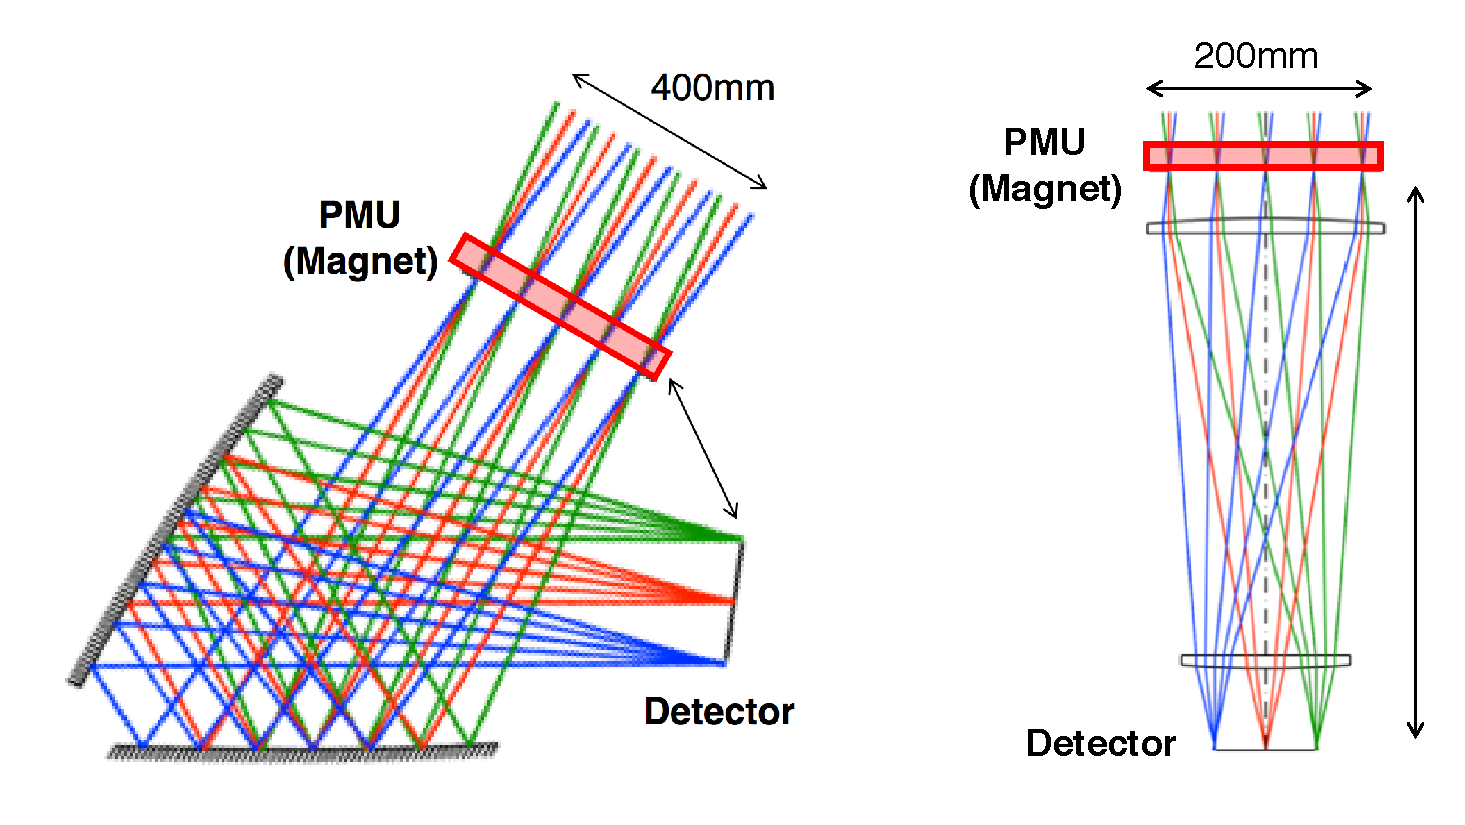
\includegraphics[width=150mm]{figs/Telescope.eps}
  \caption{}
  \label{fig:telescope}
\end{figure}

\section*{Description}

The design and the evaluation of the magnetic shield are carried out by a electromagnetic field simulation.
The software package is a finite element method (FEM) based simulation called "JMAG".
The JMAG has an advantage of a high-speed computation and containing numerous application packages of the electromagnetic field analysis.
The magnetic shielding is also included in the packages.
It has several achievements such as a design of a magnetically shielded room and so on.

At first, we must study the necessity of the PMU magnetic shield.
Figure \ref{fig:DT} shows the decision tree for the PMU magnetic shield.
The magnetic shield for the detector and its readout (detector magnetic shield) is to be installed by default.
However, it does not take into account the magnetic field from the PMU magnet.
The first decision point is whether the detector magnetic shield is sufficient or not.
We estimate the magnetic field due to the PMU magnet at the detector position by the JMAG simulation.
In this simulation,  the PMU magnet is formed into a ring shape with $\phi$=400~mm and magnetized in the axial direction.
The detector magnetic shield, whose specifications (a shape and a material) are already designed, are given to the simulation.
From the simulation result, we determine the first decision point.
If it is sufficient, there is no necessity of the PMU magnetic shield.

\begin{figure}[htbp]
  \centering
  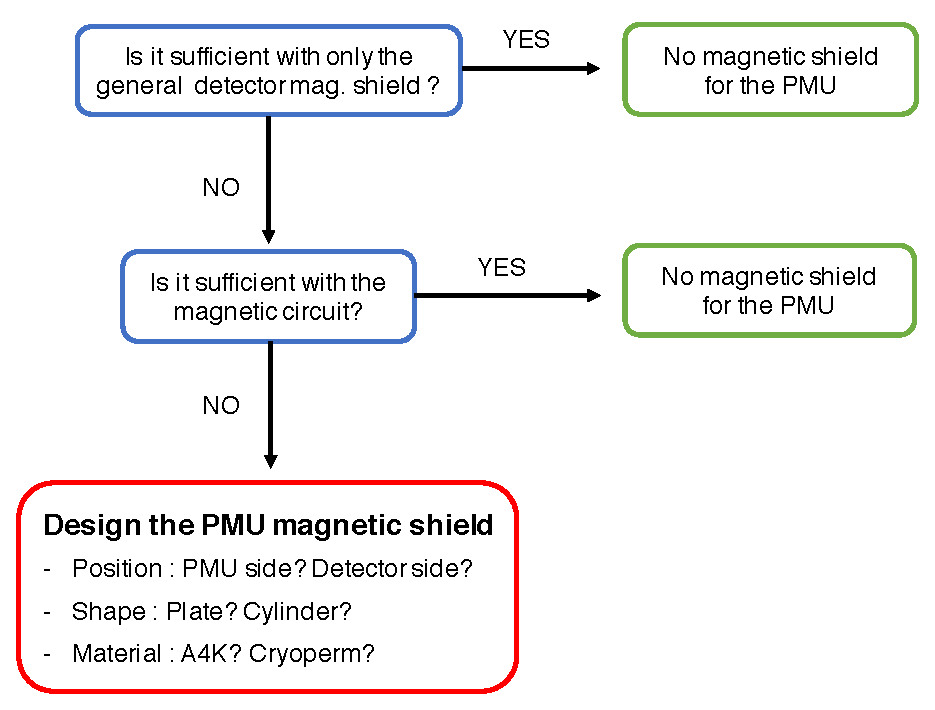
\includegraphics[width=100mm]{figs/MagShieldDecisionTree.eps}
  \caption{Decision tree and design items for the PMU magnetic shield.}
  \label{fig:DT}
\end{figure}

Then, we investigate the magnetic circuit of the PMU magnet.
The magnetic circuit is a combination of the magnetization and the yoke.
It has a possibility to reduce the magnetic field leakage due to the PMU magnet.
Figure \ref{fig:MC} shows the magnet with axial magnetization and an alternative magnetic circuit.
The alternative one has a magnet with radial magnetization and two iron yokes on both inner and outer side.
It improves not only the magnetic shielding but also the performance of the SMB.
We perform the same simulation as above with this magnetic circuit.
Then, we decide to the necessity of the PMU magnetic shield.

\begin{figure}[htbp]
  \centering
  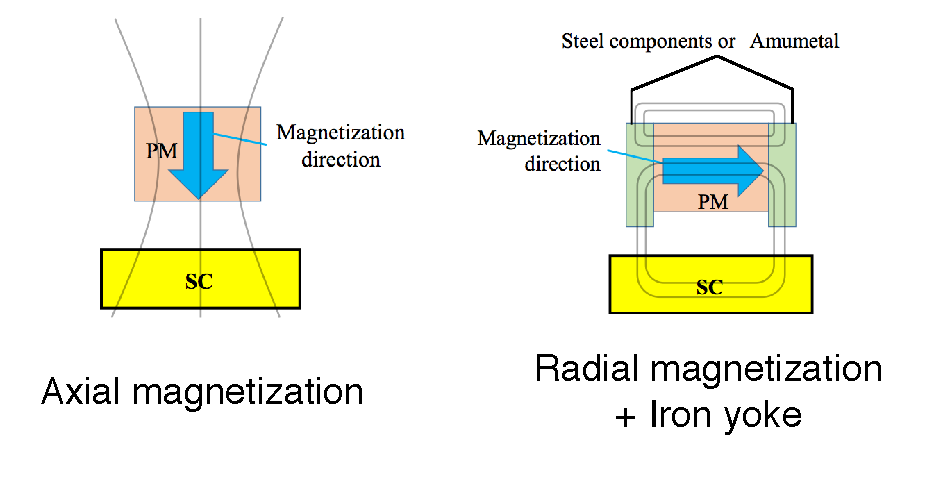
\includegraphics[width=100mm]{figs/MagneticCircuit.eps}
  \caption{}
  \label{fig:MC}
\end{figure}

If the two decision points are passed, the PMU magnetic field must be constructed.
In order to design it, we must determine mainly three design parameters as following,
\begin{itemize}
 \item Position: PMU side or detector side
 \item Shape: plate or cylinder or cylinder + bottom plate
 \item Material: A4K, Amunickel, Cryoperm10, e.t.c.
\end{itemize}
There is a trade-off between a shielding power and a weight.
We perform the simulation with their all combinations in order to select the best configuration.
The final design of the PMU magnetic shield is determined with including an interface with other equipments.

Simultaneously designing the magnetic shield by the simulation, we also compare the simulation with the actual measurement.
The comparison is performed in order to verify material properties in the JMAG simulation.
The JMAG software does not include properties of magnetic shield materials for cryogenic temperature.
Thus, it is necessary to input properties from material specifications and to adjust with a measurement.
We start to the simple comparison at room temperature with a bar magnet and plates of magnetic shield materials.
This test is also performed using cryostat for the cryogenic properties of the materials.
Then, we perform the comparison using a PMU prototype in order to evaluate the designed magnetic shield.
The PMU prototype with the diameter of $\phi$=400~mm is currently constructing at Kavli IPMU for the development of the SMB system.


\section*{Summary}
We describe the test plan for the magnetic field for the PMU.
The JMAG electromagnetic simulation is employed to design and evaluate it.
At first, the necessity of the magnetic shield is investigated with considering the detector magnetic shield and the magnetic circuit of the PMU magnet.
Then, we design the magnetic shield by the simulation with several combinations of design parameters.
The final design is determined by a trade-off study between the shielding power and the weight of the magnetic shield.
Simultaneously, the comparison between a simulation and a measurement is performed using a small PMU prototype in order to test the designed magnetic shield.

\newpage
\section*{Comments from Reviewers}

\end{document}
